\section{Волна растяжения}

Обозначим толщину стекла~$H$.

Пусть внутренняя грань идеально свободная. Мы знаем по задаче~$3.8.5$ (Савченко), что после касания фронта волны сжатия внутренней грани стекла возмущение в стекле будет результатом наложения этой прямой волны сжатия и такой же обратной волны, но растяжения, движущейся симметрично относительно свободной грани навстречу прямой волне. Обратная волна источается как будто из точки на расстоянии~$2H$ от реального места удара.
\begin{center}
    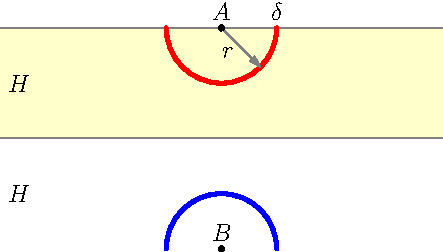
\includegraphics[]{pic2.pdf}
\end{center}
Здесь~$B$ есть мнимая точка истока обратной волны.

Не будем рассматривать тонкую область наложения прямой и обратной волн. Скажем, что через время~$\delta/(2c)$ после касания прямой внутренней грани, где $c$~--- скорость распространения волны в стекле, на расстоянии~$\delta/2$ от внутренней грани начнется появление возмущения чистого растяжения~--- это обратная волна, середина которой движется к точке удара метеорита.
\begin{center}
    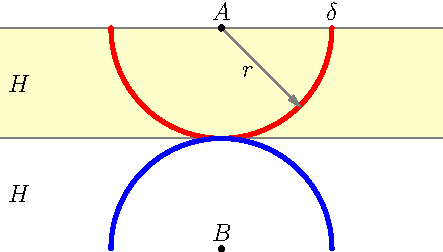
\includegraphics[]{pic3.pdf}
\end{center}
Именно с этого момента может начать разрушаться стекло через растяжение, так как прочность стекла на растяжение значительно меньше(!), чем на сжатие. Разрушение растяжением упрощенно может быть в области, где побывает только обратная волна.

В нашей модели для края разрушения растяжением (на внутренней грани стекла), толщина которого пусть~$b$, мы запишем формулу~$(1)$ применительно к обратной волне по справедливости из симметрии прямой и обратной волн:
\begin{equation*}
\boxed{\Delta P_\text{рас.$\,$max}=\sqrt{\frac{EW}{2\pi\delta}}\cdot\frac{1}{H+b}.}\tag{2}
\end{equation*}
Разделим~$(1)$ на~$(2)$ и выразим~$b$:
$$
b=\frac{\Delta P_\text{сж.$\,$max}d-\Delta P_\text{рас.$\,$max}H}{\Delta P_\text{рас.$\,$max}}.
$$

Условие существования разрушения внутри есть $b>0$, что на предыдущее накладывает
$$
\Delta P_\text{сж.$\,$max}d-\Delta P_\text{рас.$\,$max}H>0
$$
или 
$$
\boxed{d>\frac{\Delta P_\text{рас.$\,$max}}{\Delta P_\text{сж.$\,$max}}H.}
$$

При таких толщинах основного разрушения появятся разрушения на внутренней стороне.

Посмотрите, что эта модель дает близкое значение толщины откола снутри по рисунку к задаче для обычных стекол с $\dfrac{\Delta P_\text{рас.$\,$max}}{\Delta P_\text{сж.$\,$max}}\sim0{,}1$.


В книге «Физика в задачах» так же под ред. \strut О.Я. Савченко 2013 г. авторы в одной из задач предлагают тот же сюжет, но на расчет~$\dfrac{\Delta P_\text{рас.$\,$max}}{\Delta P_\text{сж.$\,$max}}$.


Посмотреть результаты экспериментов по ударам метеоритов о стекло в статье~\cite{ti76} из Новосибирска. 
